\subsubsection{Casos Bordes}

En esta secci\'on vamos a analizar ciertas familias de grafos en las cuales sabemos como se deber\'ia comportar el algoritmo exacto y que resultado tendr\'ia que devolver, para corroborar su correcto funcionamiento.
Esto no es una demostraci\'on de su correctitud, pero es una buena forma de ver si no se nos escapa la torutga.

Las familias que vamos a analizar son las siguientes:

\begin{itemize}
	\item Grafos con n nodos aisldos
	\item Grafos en forma de estrella
	\item Grafos que sean ciclos simples de n nodos
	\item Grafos completos con todos pesos 1 en sus aristas
\end{itemize}

$GRAFOS \ CON \ N \ NODOS\ AISLADOS$

Para esto generamos instancias de 0 a 100 nodos y no agergamos ninguna arista. Luego corrimos el algoritmo para k entre 2 y 50.\\
Pudimos verificar que el resultado de el algoritmo para cualquier grafo sin importar ni la cantidad de nodos, ni las particiones el resultado es siempre 0 como peso de la suma de las aristas intrapartici\'on lo cual es efectivamente cierto pues no existen aristas.\\

Corroboramos que el algoritmo exacto funciona correctamente para este tipo de instancias.

$GRAFOS\ ESTRELLA$

Para esto con el generador de instancias seleccionamos un nodo de forma aleatoria y lo conectamos al resto de los nodos.\\
Luego corrimos el algoritmo y nuevamente verificamos que se para cualquier cantidad de nodos y cualquier cantidad de particiones el peso total de la sumatoria de sus aristas es igual a 0.
Es razonable pues al nodo central se lo puede ubicar en alguna particion y al resto en cualquier otra, con lo cual no hay aristas intraparticion.

$CICLOS\ SIMPLES\ (C_n)$

Generamos grafos que eran ciclos de n elementos. Y esperabamos que tambien nos de 0 la sumatoria de las aristas sin importar la cantidad de nodos ni las particiones. Pero nos olvidamos que los ciclos simples de longitud impar no eran bipartitos. Con lo cual para cualquier grafo que sea un ciclo de longitud impar si corro el algoritmo para encontrar una 2-particion m\'inima esta nunca va a ser 0.

Pudimos corroborar que para todos los grafos que sean circuitos simples para cualquier k mayor o igual a 3 su k-PMP es 0. Y para todos los que sean circuitos simples de longitud impar y para una 2-particion la sumatoria de sus aristas intraparticion es igual a la menor de las aristas

$ K_n\ CON\ PESOS\ 1$

Con el generador de isntancias creamos grafos completos de n elementos con todos sus pesos en 1.

Pudimos verificar que el peso de las sumatoria de sus aristas intraparticion es:

\bc
	$k * (((n\  div\  k) * ((n\  div\  k) - 1)/2)) + (n\  mod\  k) * (n\  div\  k)$
\ec

B\'asicamente esto es as\'i pues en cada partici\'on voy a tener como m\'inimo n div k nodos que se conectan todos entre todos por ser un grafo completo. Con lo cual esa partici\'on va a aportar ((n div k) * ((n div k) - 1)/2) al peso total pues todas sus aristas intraparticion pesan 1. Luego tengo k particiones y por ultimo el resto de dividir a n por k son los nodos que me restan que los tengo que ubicar en alguna particion y estos se conectan con el resto de los nodos de esa particion.


\subsubsection{Rendimiento}

Para el análisis de rendimiento, corrimos el algoritmo variando la cantidad de particiones de 2 a 7, 100 instancias aleatoreas para cada n entre 5 y 20 de las cuales sacamos el promedio de tiempos, para las tres familias de grafos con el 15\%, 50\% y 100\% de sus aristas, tanto con el algoritmo sin podas y con podas.

La idea que tenemos es que el exacto sin podas al recorrer el arbol entero de solucioens solo varia en funcion de n y k por las colocacioens que puede realizar y agregandole la poda tendr\'ia que najar considerablemente el tiempo pues excluye una gran cantidad de ramas de las soluciones. 

\begin{figure}[H]
\begin{center}
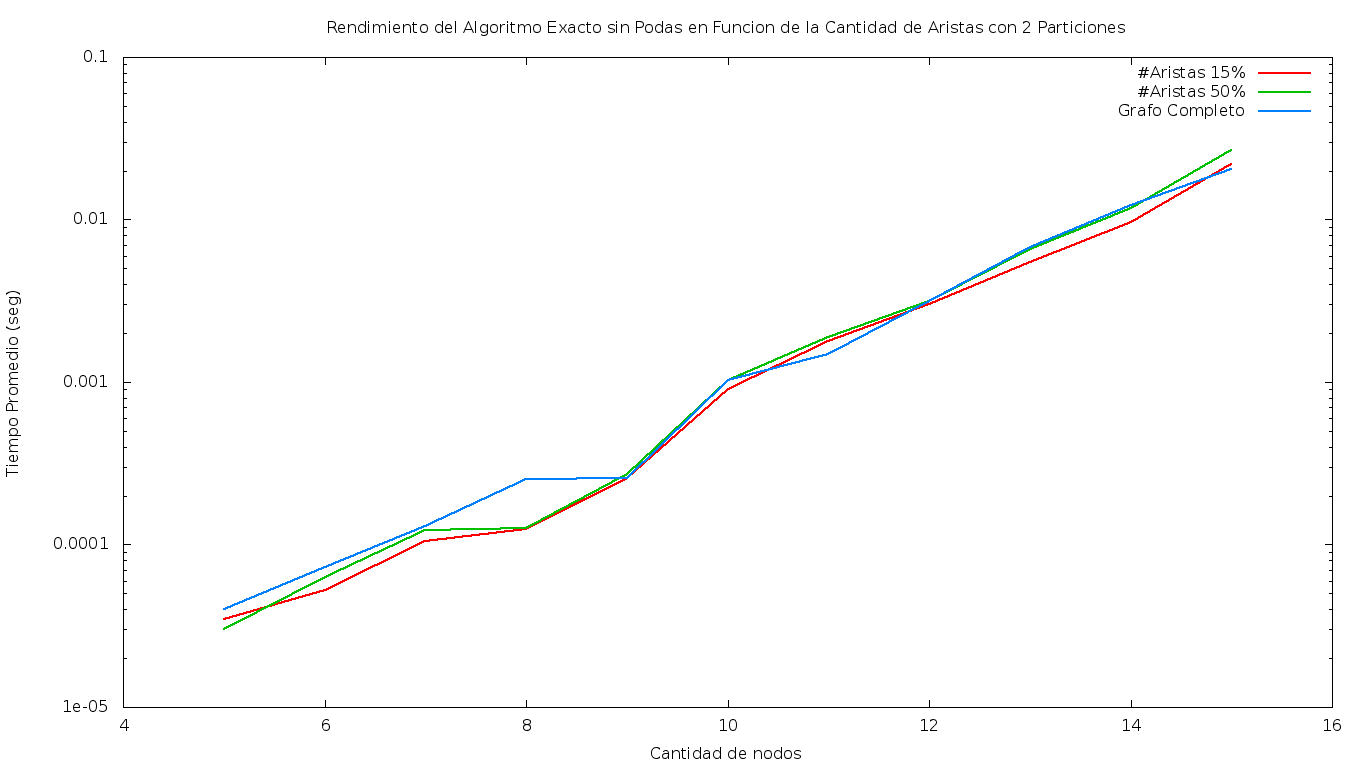
\includegraphics[scale=0.3]{finales/rendimientoExactoSinPoda2Particiones.png}
\caption{Rendimiento Exacto sin poda y K = 2}
\end{center}
\end{figure}

\begin{figure}[H]
\begin{center}
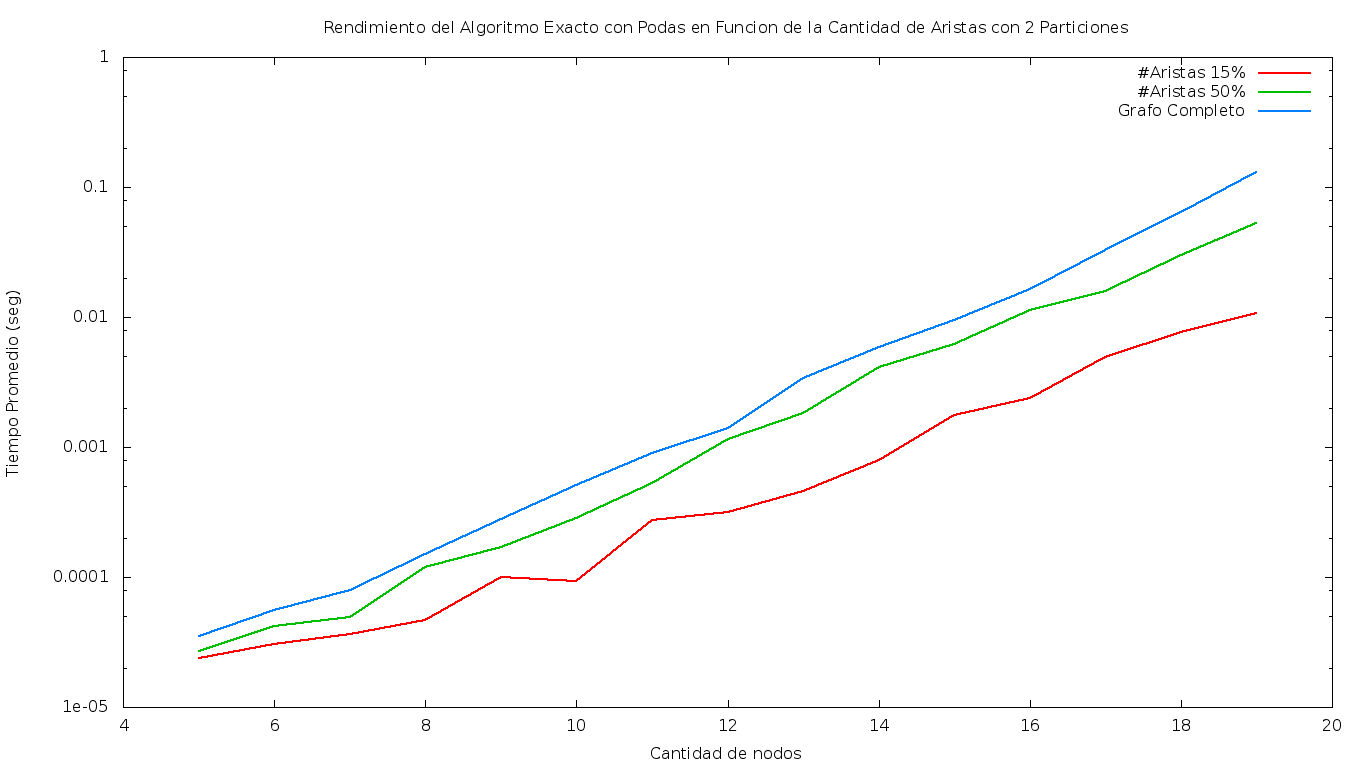
\includegraphics[scale=0.3]{finales/rendimientoExactoConPoda2Particiones.png}
\caption{Rendimiento Exacto con poda y K = 2}
\end{center}
\end{figure}

\begin{figure}[H]
\begin{center}
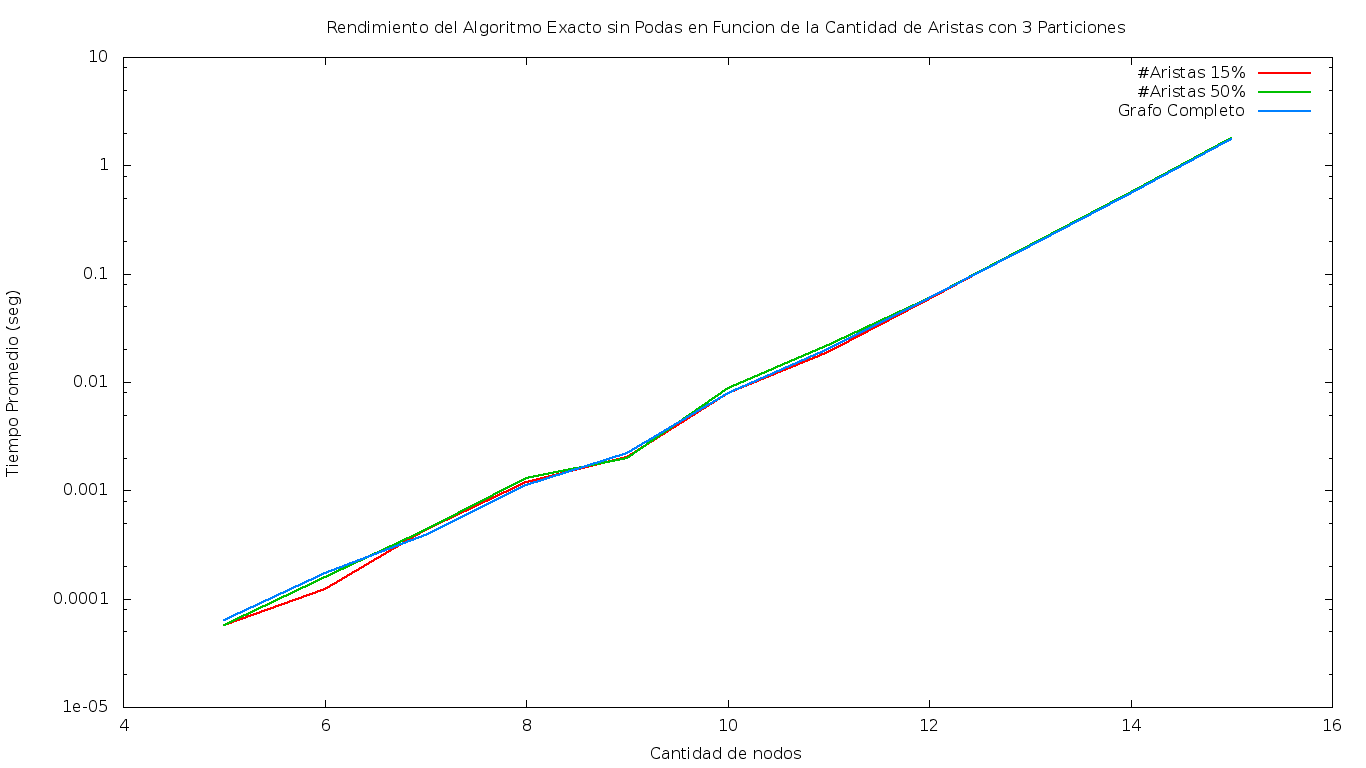
\includegraphics[scale=0.3]{finales/rendimientoExactoSinPoda3Particiones.png}
\caption{Rendimiento Exacto sin poda y K = 3}
\end{center}
\end{figure}

\begin{figure}[H]
\begin{center}
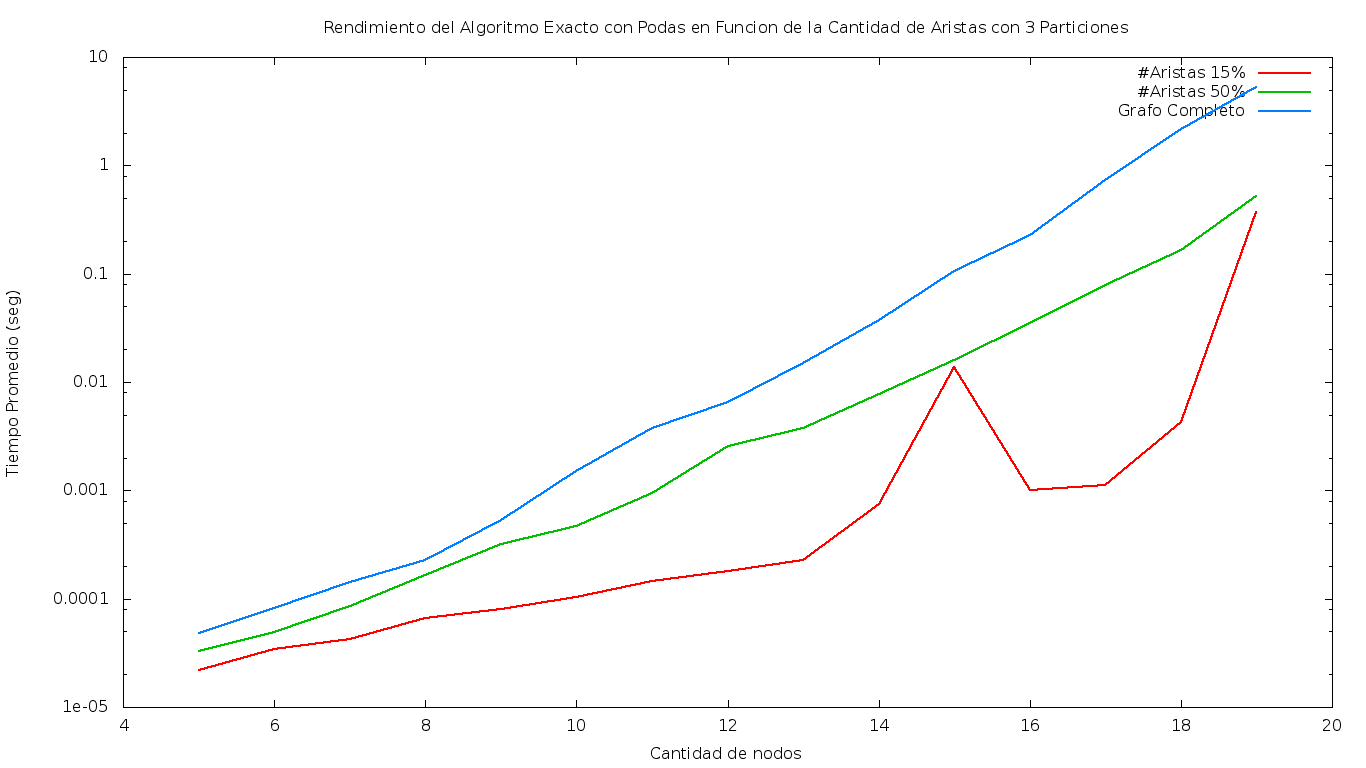
\includegraphics[scale=0.3]{finales/rendimientoExactoConPoda3Particiones.png}
\caption{Rendimiento Exacto con poda y K = 3}
\end{center}
\end{figure}

\begin{figure}[H]
\begin{center}
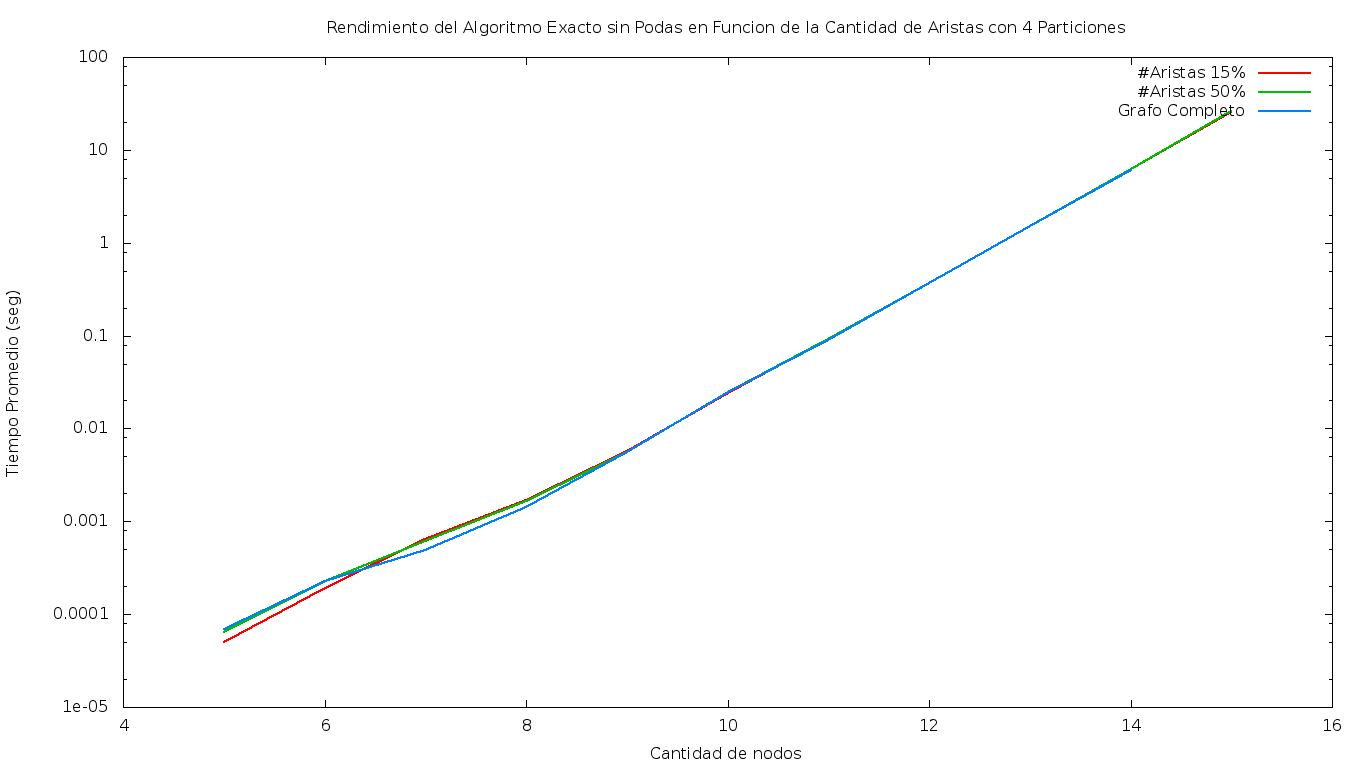
\includegraphics[scale=0.3]{finales/rendimientoExactoSinPoda4Particiones.png}
\caption{Rendimiento Exacto sin poda y K = 4}
\end{center}
\end{figure}

\begin{figure}[H]
\begin{center}
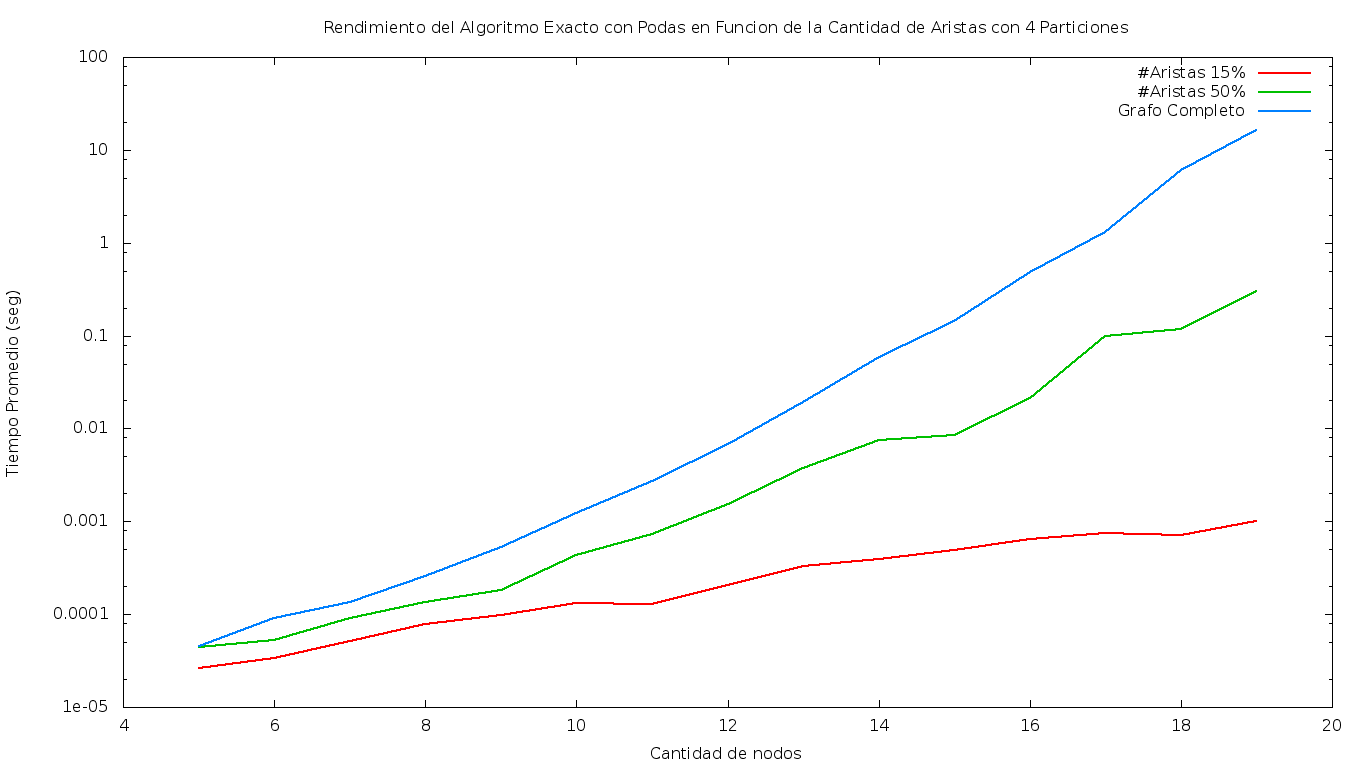
\includegraphics[scale=0.3]{finales/rendimientoExactoConPoda4Particiones.png}
\caption{Rendimiento Exacto con poda y K = 4}
\end{center}
\end{figure}

\begin{figure}[H]
\begin{center}
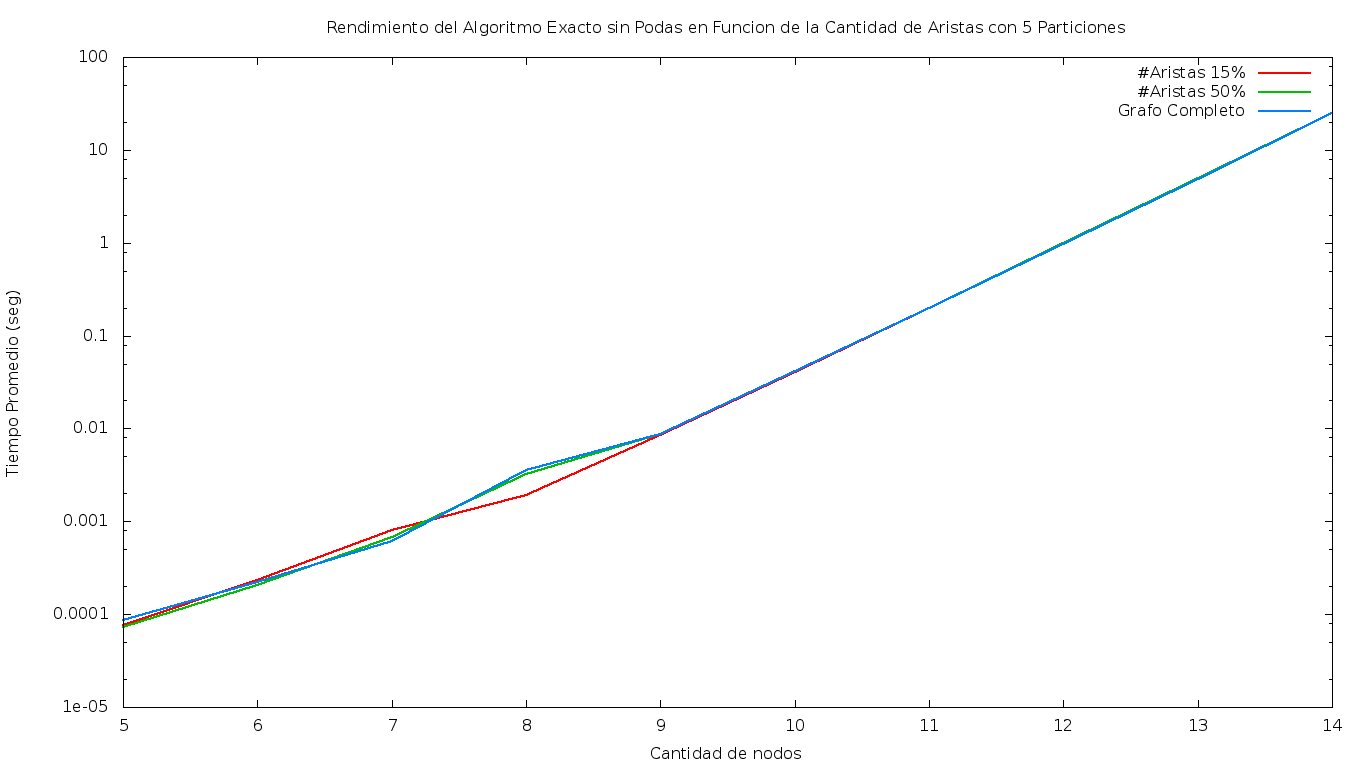
\includegraphics[scale=0.3]{finales/rendimientoExactoSinPoda5Particiones.png}
\caption{Rendimiento Exacto sin poda y K = 4}
\end{center}
\end{figure}

\begin{figure}[H]
\begin{center}
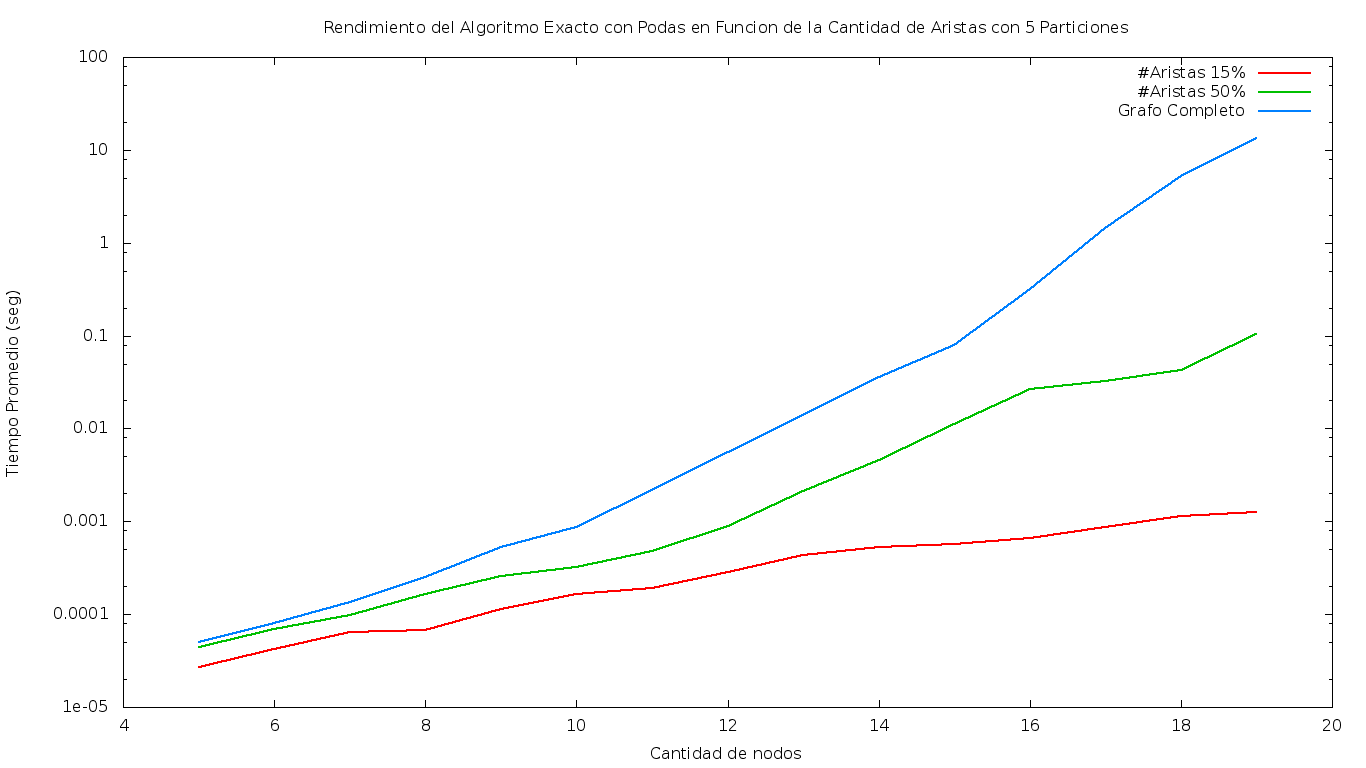
\includegraphics[scale=0.3]{finales/rendimientoExactoConPoda5Particiones.png}
\caption{Rendimiento Exacto con poda y K = 5}
\end{center}
\end{figure}

\begin{figure}[H]
\begin{center}
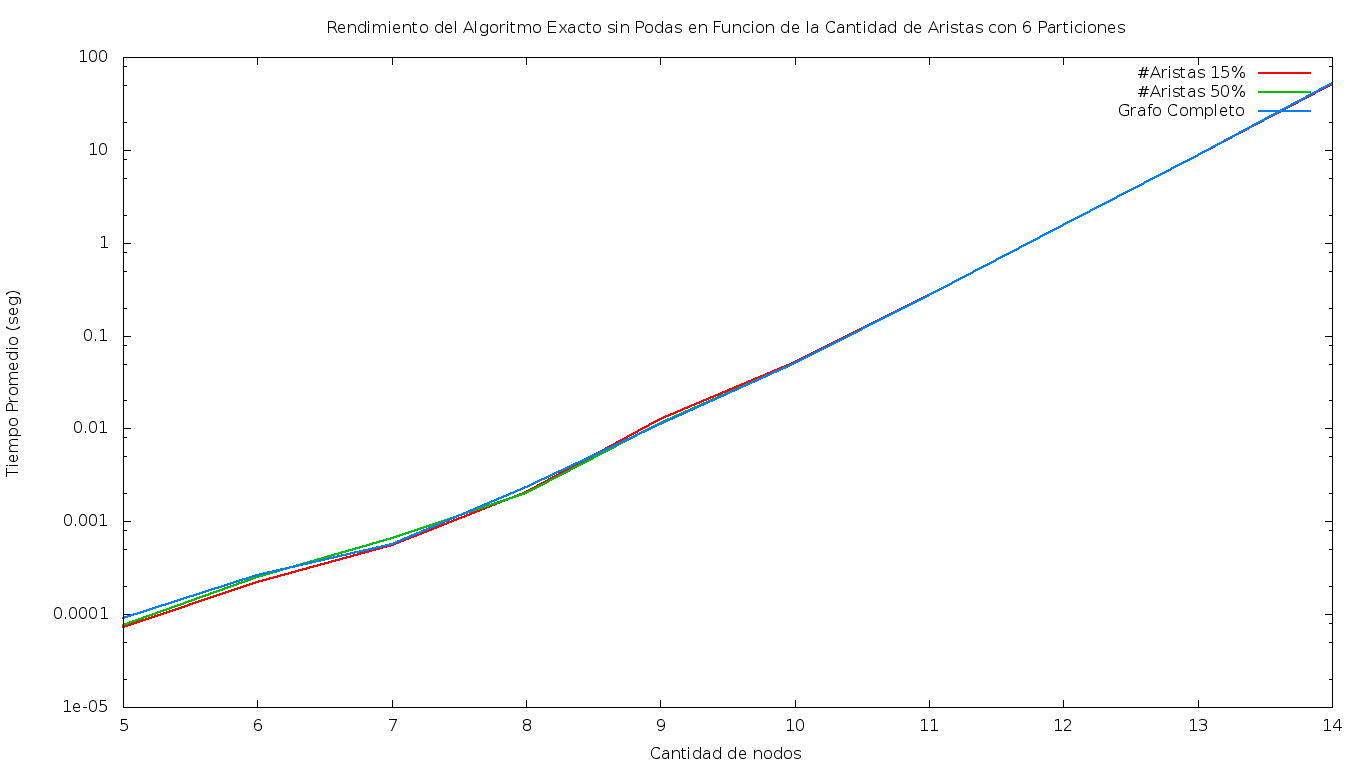
\includegraphics[scale=0.3]{finales/rendimientoExactoSinPoda6Particiones.png}
\caption{Rendimiento Exacto sin poda y K = 6}
\end{center}
\end{figure}

\begin{figure}[H]
\begin{center}
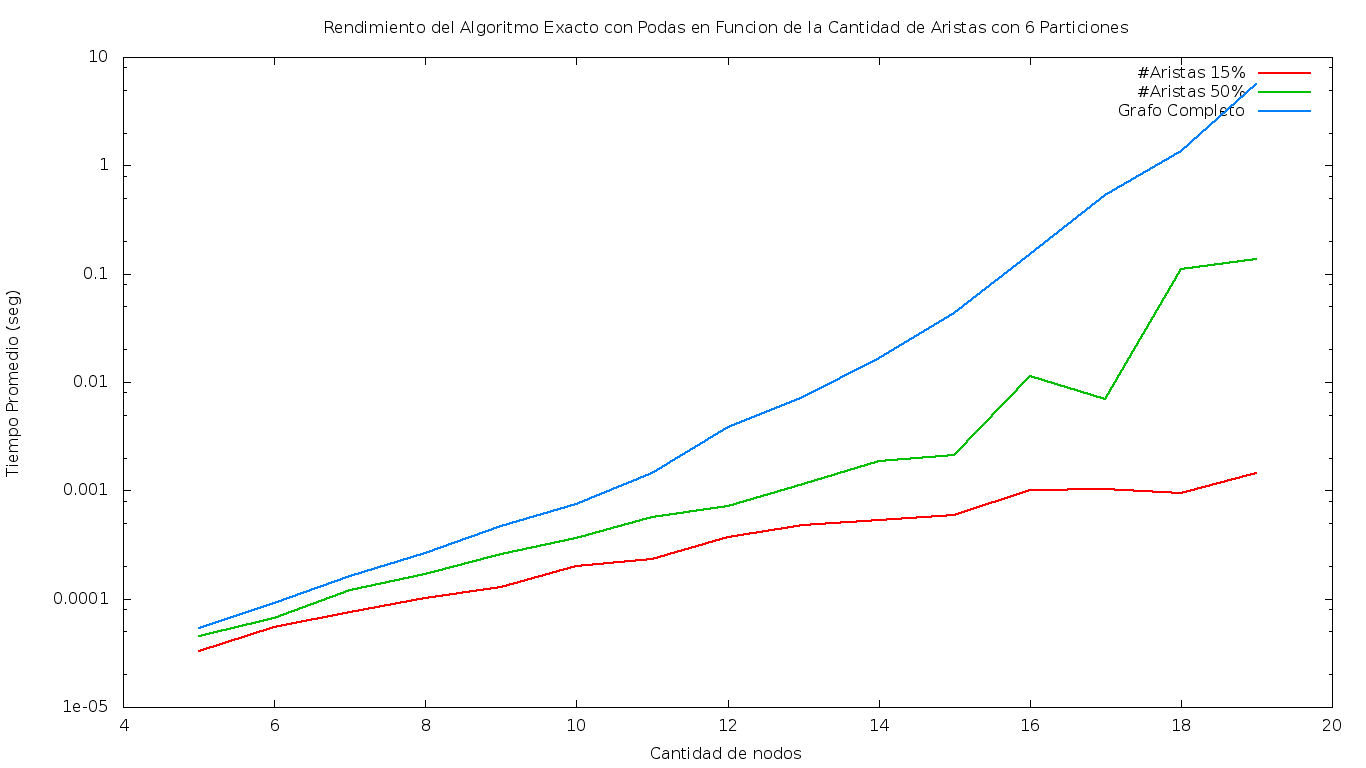
\includegraphics[scale=0.3]{finales/rendimientoExactoConPoda6Particiones.png}
\caption{Rendimiento Exacto con poda y K = 6}
\end{center}
\end{figure}

\begin{figure}[H]
\begin{center}
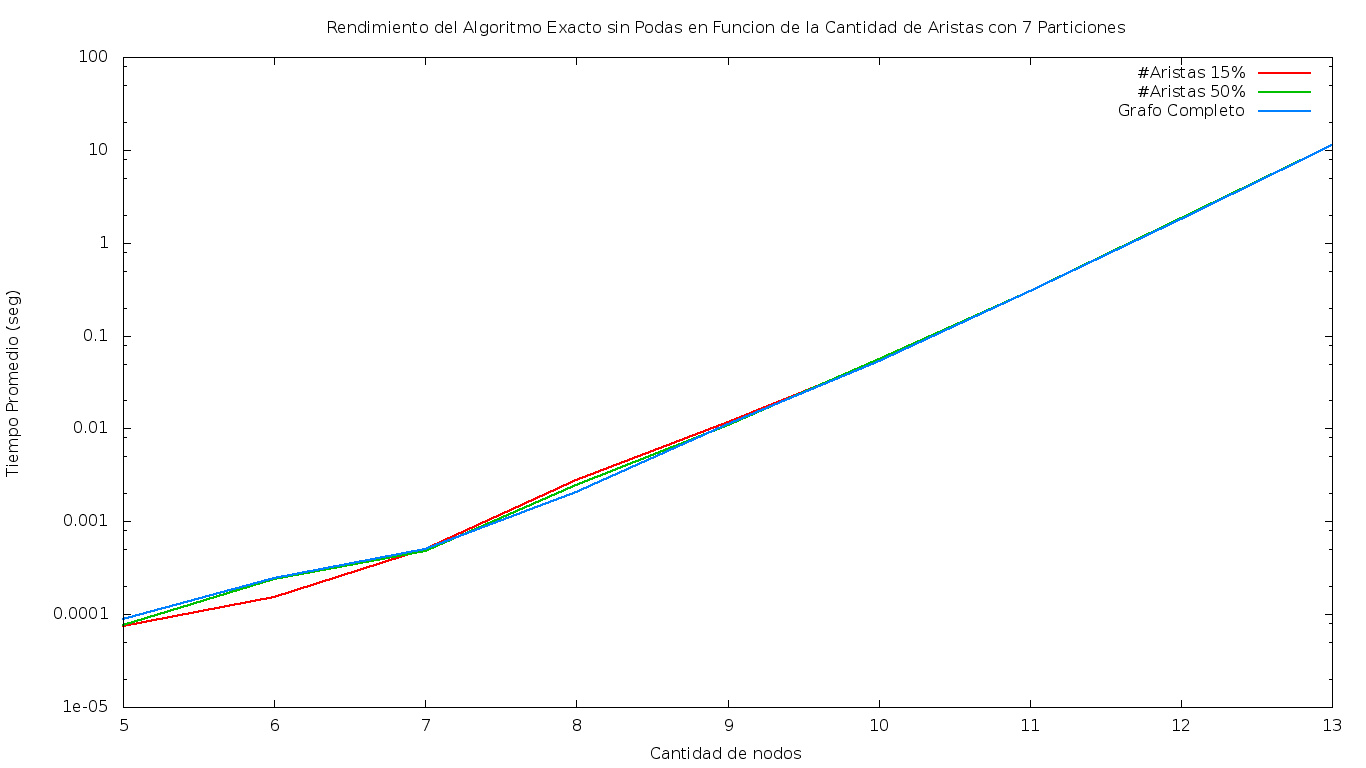
\includegraphics[scale=0.3]{finales/rendimientoExactoSinPoda7Particiones.png}
\caption{Rendimiento Exacto sin poda y K = 7}
\end{center}
\end{figure}

\begin{figure}[H]
\begin{center}
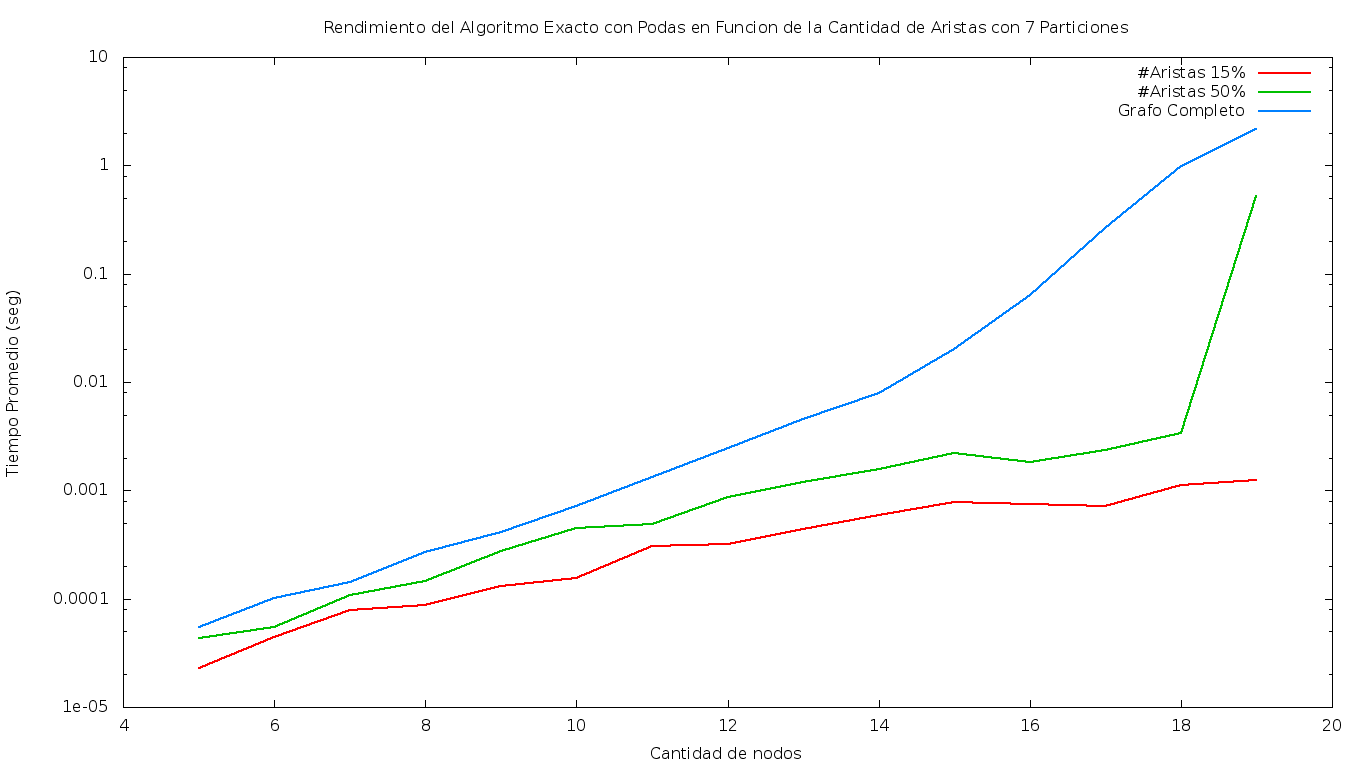
\includegraphics[scale=0.3]{finales/rendimientoExactoConPoda7Particiones.png}
\caption{Rendimiento Exacto con poda y K = 7}
\end{center}
\end{figure}


Primero algo que podemos apreciar r\'apidamente es que el algoritmo exacto sin podas no es afectado por la cantida de aristas del grafo. Se comporta de la misma manera para el 15\% de las aristas como para el 100\% Algo que era de esperarse.

Luego podemos ver que ya para valores de 15 nodos el exacto sin poda contra el mismo con las podas difiere en dos ordendes de magnitud para cualquier k particion que se tome.

Y por otro lado podemos ver como al ir aumentando la cantida de particiones en funcion que aumenta la cantidad de nodos, el algoritmo con podas al principio diverge en 1 orden de magnitud con los grafos del 15\% de aristas contra los del 100\% y para 7 particiones vemos que la diferencia es de alrededor de 4 ordenes de magnitud.

La diferencia en la ejecuci\'on en base a la densidad de los grafos para el algoritmo sin podas inferimos que es producto de que tan r\'apido se puede encontrar soluciones buenas que recorten la cantidad de soluciones a recorrer. B\'asicamente con el 15\% de las aristas, r\'apidamente podemos intuir que no alcanza para que sea conexo el grafo. Menos aun cuando algun nodo tiene varias arisatas incidentes. Con lo cual esto proboca tener varias componetes conexas en el mismo grafo, que generan conjuntos independientes con aristas intrapartic\'on = 0. Se pueden  repartir los nodos que si sean conexos en las distintas particiones y el reesto agergarlos en cualquiera total no aportan peso.

